\section{Package syntax and semantics} 
\label{syntax} 

In this section, we define the syntax and semantics of the Layout 
package for SBML Level~3 Version~1. We expound on the various data types 
and constructs defined in this package, then in \sect{examples},we 
provide complete examples of using the constructs in an example SBML 
model. 

\subsection{Namespace URI and other declarations necessary for using 
this package} 
\label{xml-namespace} 

Every SBML Level~3 package is identified uniquely by an XML namespace 
URI. For an SBML document to be able to use a given SBML Level~3 
package, it must declare the use of that package by referencing its URI. 
The following is the namespace URI for this version of the Layout 
package for SBML Level~3 Version~1: 

\begin{center} 
\uri{http://www.sbml.org/sbml/level3/version1/layout/version1} 
\end{center} 

In addition, SBML documents using a given package must indicate whether 
understanding the package is required for complete mathematical 
interpretation of a model, or whether the package is optional. This is 
done using the attribute \token{required} on the \token{<sbml>} element 
in the SBML document. For the Layout Package, the value of this 
attribute must be set to \val{false}. 

The following fragment illustrates the beginning of a typical SBML model 
using SBML Level~3 Version~1 and this version of the Layout package: 



\begin{example}
<?xml version="1.0" encoding="UTF-8"?>
 <sbml xmlns="http://www.sbml.org/sbml/level3/version1/core" level="3" version="1"
   xmlns:layout="http://www.sbml.org/sbml/level3/version1/layout/version1" layout:required="false">
\end{example}

Historically, the layout package has also been used to encode the layout 
of SBML Level 2 models, there the following namespace is to be used 
within an annotation: 


\begin{center}
\uri{http://projects.eml.org/bcb/sbml/level2}
\end{center}

A minimal example would look like this: 

\begin{example}
<?xml version="1.0" encoding="UTF-8"?>
 <sbml xmlns="http://www.sbml.org/sbml/level2" level="2" version="1">
   <model>
	  <annotation>
		  <listOfLayouts xmlns="http://projects.eml.org/bcb/sbml/level2">
			 [...]
			</listOfLayouts>
		</annotation>
	 </model>
	</sbml>
\end{example}

\subsection{Coordinate System and Size} All size information given for 
layout objects are understood to be in Point (pt), which is defined to be 1/72 of an inch (0.3527777778 
mm) as in postscript. 

The layout extension uses a Cartesian coordinate system. The origin of 
the coordinate system will be in the upper left corner of the screen. 
The positive x-axis runs from left to right, the positive y-axis run 
from top to bottom and the positive z-axis points into the screen. The 
reason to have the origin in the upper left corner of the screen is that 
most 2D packages do it that way. This coordinate system is also 
right handed just like the ones in OpenGL and Java3D, which should 
facilitate 3D implementations as well. 

\subsection{Primitive data types} \label{primtypes} 

Section~3.1 of the \sbmlthreecore specification defines a number of 
primitive data types and also uses a number of XML Schema 1.0 data 
types~\citep{biron:2000}. Of the data types defined and referenced in SBML Level~3 Core, we make use of 
\primtype{integer}, \primtype{double}, \primtype{string}, 
\primtype{SId}, \primtype{SIdRef} and \primtype{IDREF}. Additionally, the 
\Layout package defines the \primtype{SpeciesReferenceRole} and uses the \primtype{xsi:type} see 
\ref{figure:layout_uml} for the interrelation between these entities. 

The \primtype{SId} type is used as the data type for the identifiers of 
all layout classes. As such they have to be unique within the model and are not allowed to conflict with \primtype{SId}s from SBML elements or any package that use the same \primtype{SId} namespace. 

\subsubsection{Type SpeciesReferenceRole} 
\label{speciesreferencerole-type} The Layout package defines a new 
enumerated type \primtype{SpeciesReferenceRole} which represents the 
role that a species takes within a reaction. It can take only one of the 
following values: 

\begin{table}[h]
	\centering
		\begin{tabular}	{ll}		
\token{substrate}, &  \token{product}, \\
\token{sidesubstrate},& \token{sideproduct}, \\
\token{modifier},& \token{activator}, \\
\token{inhibitor} & \token{undefined}.
		\end{tabular}
\end{table}

\subsubsection{Type \token{xsi:type}} 
In order to easily differentiate between \LineSegment and \CubicBezier elements, the \token{xsi:type} attribute is used with fixed values for the two classes: \val{LineSegment} for line segments and \val{CubicBezier} for splines.

 \subsection{General features} \label{general-features} This section 
describes the common classes \Point, \Dimensions and \BoundingBox that 
are used by all other classes of this package. It also describes the 
representation of curves. 

\subsubsection{The Point class} \label{point-class} 
\label{position-class} A point is specified via the required attributes 
\token{x}, \token{y} and an optional attribute \token{z}, all of which 
are of type \primtype{double}. If the attribute \token{z} is not 
specified, the object is a two dimensional object. 

The \Point class also has an optional attribute \token{id} of type 
\primtype{SId}. While not used in the \Layout package, it can be used by programs to refer to the elements. 

\begin{figure}[!h]
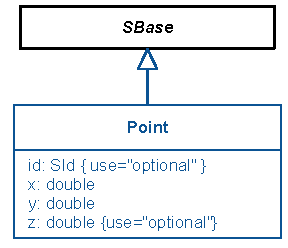
\includegraphics{uml/layout-point-uml}\\
\caption{The definitions of the \Point class.}
\label{uml:point}
\end{figure}

\subsubsection{The Dimensions class} \label{dimensions-class} A 
dimension is specified via the required attributes \token{width}, 
\token{height} and an optional attribute \token{depth}, all of which are 
of type \primtype{double}. If the attribute \token{depth} is not 
specified, the object is a two dimensional object. 

The \token{width} specifies the size of the object in the direction of 
the positive x axis, the \token{height} attribute specifies the size of 
the object along the positive y axis and the \token{depth} attribute 
specifies the size of the object along the positive z axis. All sizes 
for \Dimensions objects are positive values, and so the attributes are not allowed to take negative values. 

The \Dimensions class also has an optional attribute \token{id} of type 
\primtype{SId}. While not used in the \Layout package, it can be used by programs to refer to the elements. 


\begin{figure}[!h]
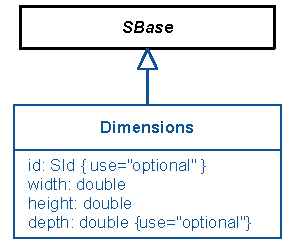
\includegraphics{uml/layout-dimensions-uml}\\
\label{uml:dimensions}
\caption{The definitions of the \Dimensions class.}
\end{figure}
 \subsubsection{The BoundingBox class} \label{boundingbox-class} A 
\BoundingBox consists of the required elements \token{position} and \token{dimensions}. 

The \BoundingBox class also has an optional attribute \token{id} of type 
\primtype{SId}. While not used in the \Layout package, it can be used by programs to refer to the elements. 

\begin{figure}[!h]
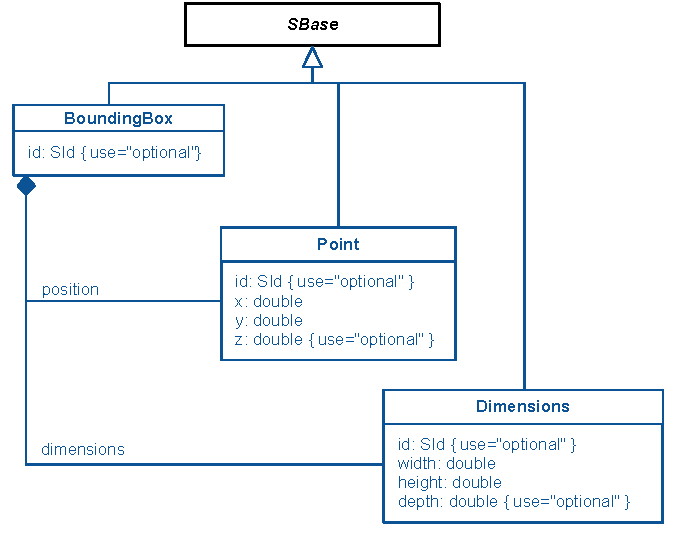
\includegraphics{uml/layout-boundingbox-uml}\\
\label{uml:boundingbox}
\caption{The definitions of the \BoundingBox class.}
\end{figure}

\paragraph{The \token{position} element} The \token{position} always 
specifies the upper left corner of the bounding box. The 
\token{position} is of type \Point. 

\paragraph{The \token{dimensions} element} The \token{dimensions} 
element is required and of type \Dimensions. It represents the size of
the bounding box.

\subsubsection{The Curve class } \label{curve-class} The curve class 
describes how to connect elements of the layout package. It is fully 
specified by a mandatory \token{listOfCurveSegments} element and is used 
in four places: 

\begin{itemize}

	\item {\SpeciesReferenceGlyph: Here it describes a curve from/to 
	the center piece of the parent \ReactionGlyph to/from the 
	\SpeciesGlyph it represents.}
	\item {\ReactionGlyph: Here it describes a curve for the 
	center piece of a reaction. }	
	\item {\ReferenceGlyph: Here it describes a curve from / to 
	the center piece of the parent \GeneralGlyph to/from the glyph 
	it represents.}
	\item {\GeneralGlyph: Here it describes a curve for the 
	center piece of an additional relationship. }	
	
\end{itemize}

In the above the \textit{center piece} refers to either the \Curve element of a \ReactionGlyph, or its \BoundingBox. 

\begin{figure}[!h]
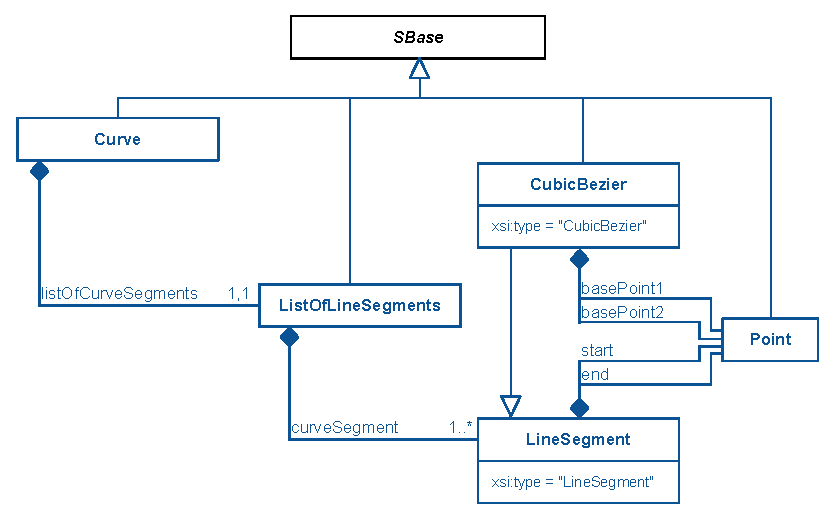
\includegraphics{uml/layout-curve-uml}\\
\caption{The definitions of the \Curve class.}
\label{uml:curve}
\end{figure}

\paragraph{The \token{listOfCurveSegments} element} 
\label{listofcurvesegments-class} 

The \token{listOfCurveSegments} contains an arbitrary number of curve 
segments that can be either of type \LineSegment or of type 
\CubicBezier. 


\subsubsection{The LineSegment class} 
\label{linesegment-class} 

The \LineSegment class consists of the mandatory attribute 
\token{xsi:type} and two elements of type \Point. One is called 
\token{start} and represents the starting point of the line, the other 
is called \token{end} and represents the endpoint of the line. 

\paragraph {The \token{xsi:type} attribute} For straight line segments, 
the attribute \token{xsi:type} must have the value set to: 

\begin{center}
\val{LineSegment}
\end{center}

Note that the \token{xsi:type} is from the \token{xsi} namespace: 

\begin{center}
\val{http://www.w3.org/2001/XMLSchema-instance}
\end{center}

\subsubsection{The CubicBezier class}
\label{cubicbezier-class}
In order to be able to represent smooth curves the \Layout package defines the class \CubicBezier. It represents a Bezier curve (\cite{beziercurve}), as is readily available in most Graphic APIs. 

The class \CubicBezier is derived from \LineSegment. It consists of 
the four elements, the two inherited elements \token{start} and \token{end}, that specify the starting point and the endpoint of the cubic bezier curve, and two elements \token{basePoint1} and \token{basePoint2} specify two additional base points that are needed to describe a cubic bezier curve. 

\begin{figure}[!h]
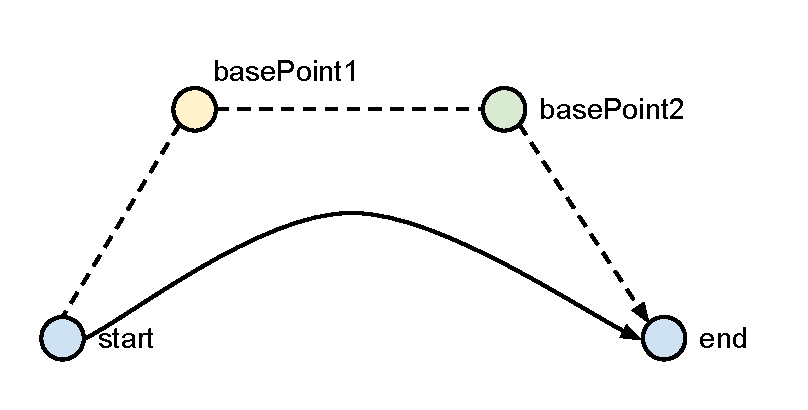
\includegraphics{figures/layout-cubic-bezier}\\
\caption{A depiction of a cubic bezier curve, including the points \token{start}, \token{end} as well as \token{basePoint1} and \token{basePoint2}.} 
\label{figure:cubic-bezier}
\end{figure}


The \token{basePoint1} element represents the base point closer to the \token{start} point and \token{basePoint2} the base point closer to \token{end} point. This allows tools not able to render bezier curves to approximate them by directly connecting the four points (as visible in the dashed line in \ref{figure:cubic-bezier}). 


\paragraph {The \token{xsi:type} attribute} For cubic bezier curves, the 
attribute \token{xsi:type} must have the value set to: 


\begin{center}
\val{CubicBezier}
\end{center}

Note that the \token{xsi:type} is from the \token{xsi} namespace: 

\begin{center}
\val{http://www.w3.org/2001/XMLSchema-instance}
\end{center}

\subsection{The extended Model class}
\label{model-class}

The \SBML \Model class is extended with the addition of one child the 
\token{listOfLayouts}. A \Model may contain at most one such list. 


\begin{figure}[!h]
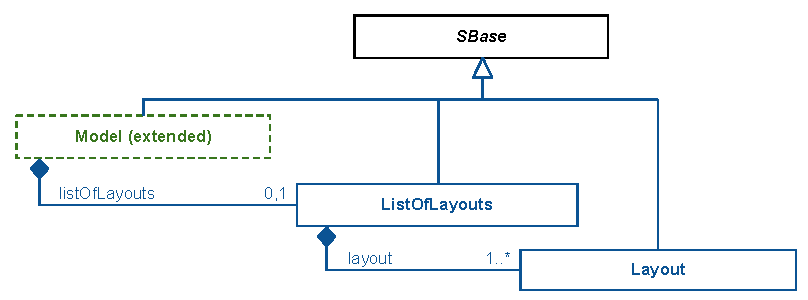
\includegraphics{uml/layout-extended-model-uml}\\
\caption{The definitions of the extended \Model class.}
\label{figure:extendedmodel}
\end{figure}

\paragraph{The listOfLayouts class}
\label{listoflayouts-class}
As shown in \ref{figure:extendedmodel} the \ListOfLayouts is derived from 
\SBase and inherits the attributes \token{metaid} and \token{sboTerm}, 
as well as the subcomponents for \Annotation and \Notes. The 
\ListOfLayouts must contain at least one \Layout (defined in 
\ref{layout-class}). 


\subsection{The Layout class}
\label{layout-class}
The layout class stores layout information for some or all elements of 
the SBML model as well as additional objects that need not be connected 
to the model. 

The \LayoutClass has two attributes: \token{id} and 
\token{name}. Additionally a \Dimensions element specifies the size of 
the layout. The actual layout elements are contained in several lists 
namely: a \ListOfCompartmentGlyphs, a \ListOfSpeciesGlyphs, a 
\ListOfReactionGlyphs, a \ListOfTextGlyphs, and a 
\ListOfAdditionalGraphicalObjects. Each of these lists can only occur 
once, and, if present, is not allowed to be empty. 


\begin{figure}[!h]
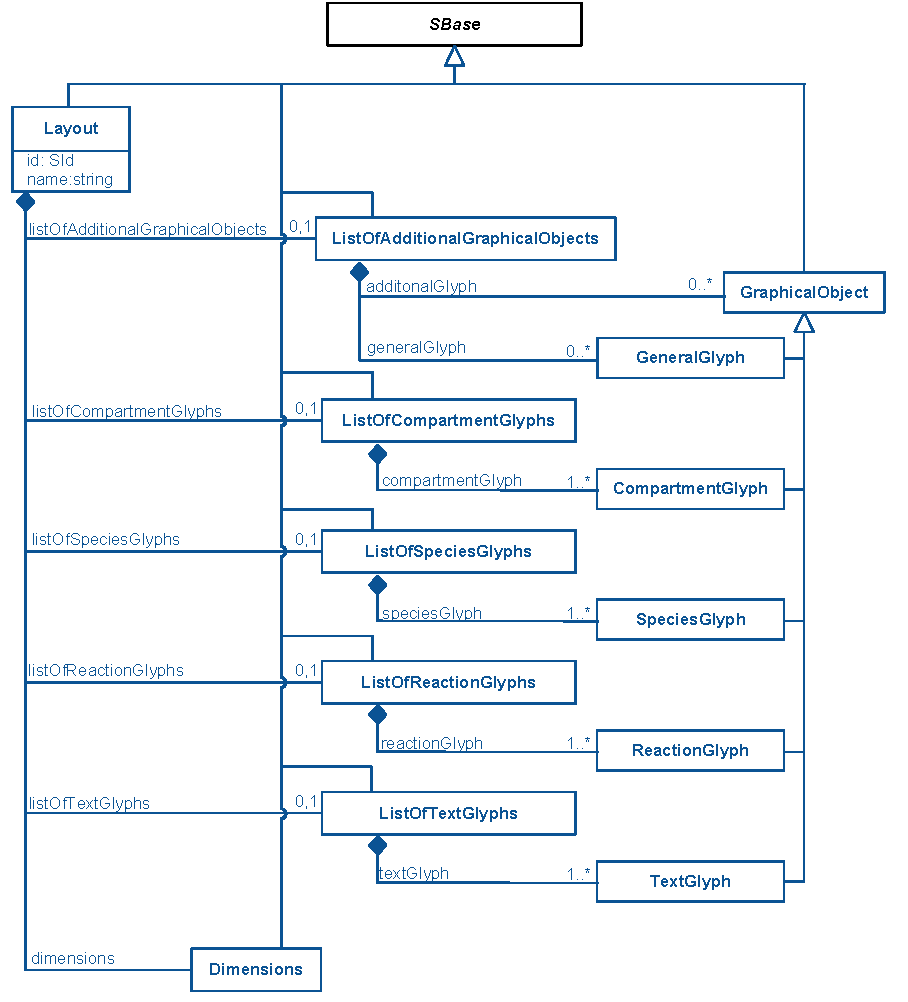
\includegraphics{uml/layout-layout-uml}\\
\caption{A UML representation of the \LayoutPackage. Derived from 
\SBase, the \Layout classes inherit support for constructs such as SBML 
\Notes and {\Annotation}s. See \ref{conventions} for conventions related 
to this figure. The individual classes are further discussed in the 
text.} 
\label{figure:layout_uml}
\end{figure}

\paragraph{The \token{id} attribute}
The \token{id} attributes takes a required value of type \primtype{SId}. 
The \token{id} which uniquely identifies the layout. 


\paragraph{The \token{name} attribute}
The \token{name} attributes takes an optional value of type 
\primtype{String}. It allows to specify a human readable name for the 
\LayoutClass. 


\paragraph{The \token{dimensions} element}
The \token{dimensions} element of type \Dimensions specifies the 
dimensions of this layout. This element is required. It holds the 
dimensions of all layout elements (care should be taken when using cubic 
beziers (see \ref{cubicbezier-class}, that the described curve also lies 
within the given dimensions). 


\paragraph{The \token{listOfCompartmentGlyphs} element}
\label{listofcompartmentglyphs-class}
The \token{listOfCompartmentGlyphs}, when present must contain one or 
more \CompartmentGlyph elements. 

Note that not all \Compartment elements have to be represented by a \CompartmentGlyph. In fact quite often the 
compartment is omitted in a layout for a uni-compartmental network. 


\paragraph{The \token{listOfSpeciesGlyphs} element}
\label{listofspeciesglyphs-class}
The \token{listOfSpeciesGlyphs}, when present must contain one or more 
\SpeciesGlyph elements. Just as with \CompartmentGlyph elements, not every \Species of the model has to have a representation in this list.


\paragraph{The \token{listOfReactionGlyphs} element}
\label{listofreactionglyphs-class}
The \token{listOfReactionGlyphs}, when present must contain one or more 
\ReactionGlyph elements. Similar as with \ListOfCompartmentGlyphs and 
\ListOfSpeciesGlyphs, not all reactions of the containing SBML model 
have to be included in the containing layout. 


\paragraph{The \token{listOfTextGlyphs} element}
\label{listoftextglyphs-class}
The \token{listOfTextGlyphs}, when present, must contain one or more 
\TextGlyph elements. 


\paragraph{The \token{listOfAdditionalGraphicalObjects} element}
\label{listofadditionalgraphicalobjects-class}
Most objects for which layout information is to be included in an SBML 
file have a corresponding object in the SBML model. As there might be 
cases where the user wants to include object types in the layout that do 
fall in any of the other categories described below, we include a 
\token{listOfAdditionalGraphicalObjects} in each \Layout object. This 
list holds an arbitrary number of \token{graphicalObject} elements. The 
\token{graphicalObject} only defines a bounding box in a specific place 
in the layout without giving additional information about its contents. 

The \token{listOfAdditionalGraphicalObjects}, when present must contain 
one or more of the following elements: \GraphicalObject, \GeneralGlyph. 

When using a \GraphicalObject it is recommended that some form of meta 
information is provided. For additional relationships such as SBML events or rules, the \GeneralGlyph can be used, see \ref{generalglyph-class}. 


\subsection{The GraphicalObject class} 
\label{graphicalobject-class}
All the more specific layout elements (\CompartmentGlyph, \GeneralGlyph, 
\SpeciesGlyph, \ReactionGlyph, \ReferenceGlyph, \TextGlyph, and 
\SpeciesReferenceGlyph) are derived from \GraphicalObject. 

Each GraphicalObject has a \BoundingBox, which specifies the position 
and the size of the object. 


\begin{figure}[!h]
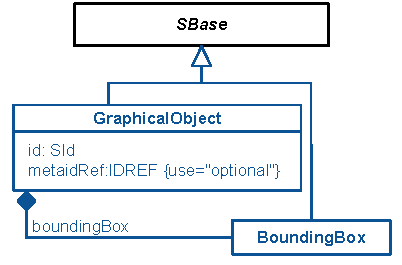
\includegraphics{uml/layout-graphicalobject-uml}\\
\label{uml:graphicalobject}
\caption{The definitions of the \GraphicalObject class.}
\end{figure}

Programs are encouraged to use annotations to \GraphicalObject elements 
in the \token{listOf\-Additional\-Graphical\-Objects} that describe program 
specific graphical information. 



\paragraph{The \token{id} attribute}
The \GraphicalObject has a mandatory \token{id} attribute of type 
\primtype{SId} through which it can be identified. 


\paragraph{The \token{metaidRef} attribute}
The \GraphicalObject has an optional \token{metaidRef} attribute of type 
\primtype{IDREF} that allows the object to uniquely reference elements in the \Model. 
Wherever possible it is preferred that the more specific reference 
mechanisms are being used. 


\subsection{The CompartmentGlyph class }
\label{compartmentglyph-class}
The \CompartmentGlyph class is derived from \GraphicalObject and inherits its attributes. Additionally, it has two optional attributes 
\token{compartment} and \token{order}. For an example see \ref{example:compartmentglyph}.


\begin{figure}[!h]
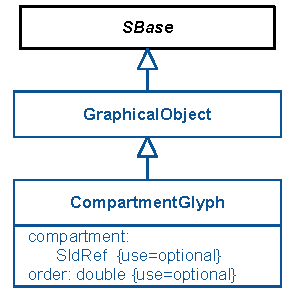
\includegraphics{uml/layout-compartmentglyph-uml}\\
\label{uml:compartmentglyph}
\caption{The definitions of the \CompartmentGlyph class.}
\end{figure}


\paragraph{The \token{compartment} attribute}
The \token{compartment} attribute is of type \primtype{SIdRef}. It 
is used to add a reference to the \token{id} of the corresponding 
compartment in the model. Since the \token{compartment} is optional, the 
user can specify compartments in the layout that are not part of the 
model. 

\paragraph{The \token{order} attribute}
The \token{order} attribute is an optional attribute of type 
\primtype{double}. It is there to handle the case where compartments in a layout are overlapping, and tools would want to clearly disambiguate which \CompartmentGlyph is on top of another one. 

The \token{order} attribute follows the coordinate system. There 
the \token{z} dimension is pointing into the screen, thus an element 
with a \textbf{lower} \token{order} value will be \textbf{in front} of 
elements with a \textbf{higher} value.

If not specified, the \token{order} is undefined and tools are free to 
display the compartment glyphs in the order that best fits their needs. 

\subsection{The SpeciesGlyph class}
\label{speciesglyph-class}
In addition to the attributes from \GraphicalObject, the \SpeciesGlyph 
object has an optional \token{species} attribute. For an example see \ref{example:speciesglyph}.

\begin{figure}[!h]
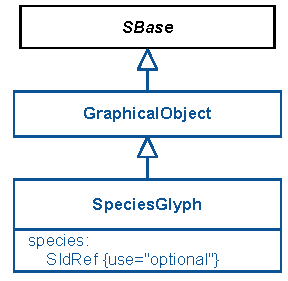
\includegraphics{uml/layout-speciesglyph-uml}\\
\label{uml:speciesglyph}
\caption{The definitions of the \SpeciesGlyph class.}
\end{figure}

\paragraph{The \token{species} attribute}
The \token{species} attribute of type \primtype{SIdRef} allows modelers to link the \SpeciesGlyph to the \token{id} of the corresponding species object  in the \Model. The \token{species} attribute is optional to allow the  program to specify species representations that do not have a direct  correspondence in the model. This might be useful if some pathway has been collapsed, but is still treated by layout programs. 


\subsection{The ReactionGlyph class}
\label{reactionglyph-class}
The \ReactionGlyph is used to represent \Reaction elements in the 
layout. Analogous to how a \Reaction object has to at least have one reactant 
or product, the \ReactionGlyph has to at least have one 
\SpeciesReferenceGlyph stored in the \ListOfSpeciesReferenceGlyphs. 

The \ReactionGlyph inherits from \GraphicalObject. In addition to the attributes inherited from \GraphicalObject, the 
\ReactionGlyph is described by an attribute \token{reaction}, a \Curve 
element and a \token{listOfSpeciesReferenceGlyphs} element. 

The \Curve describes the center section of a \ReactionGlyph. The center section is frequently used by tools to separate the point where substrates arcs come together, from the point where product arcs split off. The \Curve is optional, and when not present the dimensions of the inherited \BoundingBox describes the center section, by storing its position and dimension. 

For an example see \ref{example:reactionglyph}. 


\begin{figure}[!h]
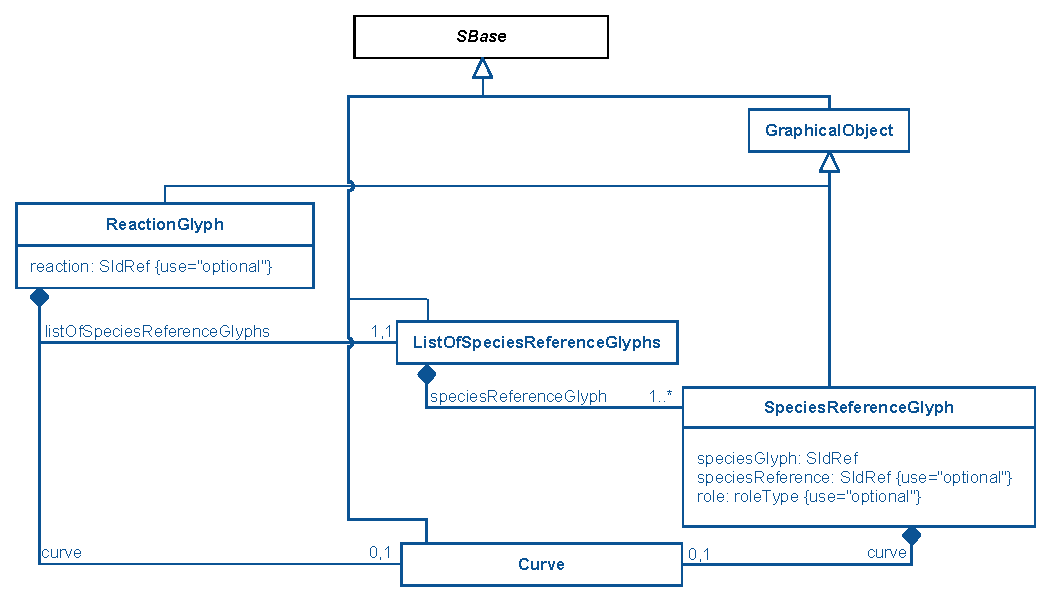
\includegraphics{uml/layout-reactionglyph-model-uml}\\
\label{uml:reactionglyph}
\caption{The definitions of the \ReactionGlyph class.}
\end{figure}

\paragraph{The \token{reaction} attribute}
The \token{reaction} attribute of type \primtype{SIdRef} is used to 
specify the \token{id} of the corresponding \Reaction in the model. This 
reference is optional. 


\paragraph {The \token{listOfSpeciesReferenceGlyphs} element}
\label{listofspeciesreferenceglyphs-class}
Since a \Species element can have several graphical representations in 
the layout there must be a way to specify which \SpeciesGlyph should be 
connected to the \ReactionGlyph. This is done using the 
\token{listOfSpeciesReference\-Glyphs}. 

The \ListOfSpeciesReferenceGlyphs is mandatory, since every \Reaction 
has to have at least one reactant or product. 


\paragraph {The \token{curve} element}
The optional \Curve element (\ref{curve-class}) can be used to describe 
a curve representation for the \ReactionGlyph. 

If a \ReactionGlyph specifies a curve, the bounding box is to be 
ignored. 


\subsubsection{The SpeciesReferenceGlyph class}
\label{speciesreferenceglyph-class}
The \token{speciesReferenceGlyph} element describes the graphical 
connection between a \SpeciesGlyph and a \ReactionGlyph (which would be 
an arrow or some curve in most cases). 

As can be seen in the diagram \ref{uml:reactionglyph}, a 
\SpeciesReferenceGlyph inherits from \GraphicalObject. Additionally, it 
has a mandatory attribute \token{speciesGlyph} and two optional 
attributes \token{speciesReference} and \token{role}. Optionally, the 
\SpeciesReferenceGlyph also has an element \token{curve}. 

If the \token{curve} is specified, it overrides the inherited bounding box.


\paragraph{The \token{speciesGlyph} attribute}
The \token{speciesGlyph} is of type \primtype{SIdRef}. It contains a 
reference to the \token{id} of a \SpeciesGlyph object that is to be 
connected to the \ReactionGlyph. 

This attribute is mandatory so as to ensure unambiguity about which SpeciesGlyph has to be connected with this ReactionGlyph. 


\paragraph{The \token{speciesReference} attribute}
The \token{speciesReference} is an optional attribute of type 
\primtype{SIdRef} that allows modelers to connect the \SpeciesReferenceGlyph with 
a particular \SpeciesReference (or \ModifierSpeciesReference) of the 
containing model. 

NOTE: The \token{id} on a \SpeciesReference and 
\ModifierSpeciesReference was only introduced in \sbmlthreecore, in 
order to successfully use the \token{speciesReference} in prior Levels 
of SBML, the corresponding species reference has to be annotated with an 
identifier. The annotation would look like this: 


\begin{example}
	<annotation>
		<layoutId xmlns="http://projects.eml.org/bcb/sbml/level2" id="theId"/>
	</annotation>
\end{example}

This \token{id} has to be unique within the global \primtype{SId} namespace of the SBML model and can thus be used to reference a given species reference. For a complete example see also \ref{example:speciesreferenceid}. 


\paragraph{The \token{role} attribute}
\label{attribute:role}
The \token{role} attribute is of \primtype{SpeciesReferenceRole} and is 
used to specify how the species reference should be displayed. Allowed 
values are \token{substrate}, \token{product}, \token{sidesubstrate}, 
\token{sideproduct}, \token{modifier}, \token{activator}, 
\token{inhibitor} and \token{undefined}. 

This attribute is optional and should only be necessary if the optional 
\token{speciesReference} attribute is not given or if the respective 
information from the model needs to be overridden. 

\begin{itemize}

	\item { The values \token{substrate} and \token{product} are used if 
	the species reference is a main product or substrate in the reaction. } 
	\item { \token{sidesubstrate} and \token{sideproduct} are used for 
	simple chemicals like ATP, NAD+, etc. This allows programs to render 
	them as side reactions. } \item { \token{activator} and 
	\token{inhibitor} are modifiers where their influence on the reaction is 
	known and \token{modifier} is a more general term if the influence is 
	unknown or changes during the course of the simulation. } 

\end{itemize}

In order to specify more specific types of interactions it is recommended to use the \token{sboTerm} on the \SpeciesReference.

\paragraph{The \token{curve} element}
The \token{curve} is an optional element of type \Curve. When present 
the glyphs bounding box (as inherited from the \GraphicalObject) is to 
be disregarded. 

So as to make the drawing of these curves as easy as possible the line 
segments should be ordered depending on the role of the 
\SpeciesReferenceGlyph. If no \token{role} attribute is defined the role 
to be assumed is taken from the role that the \SpeciesReference 
referenced via the attribute \token{speciesReference} has, otherwise it 
is \token{undefined}. 


\begin{itemize}
	\item {\token{product}, \token{sideproduct}, \token{substrate}, 
	\token{sidesubstrate}, \token{undefined}: The line segments have their 
	\token{start} element at the \ReactionGlyph and their \token{end} 
	element at the \SpeciesGlyph.} 
	\item {\token{activator}, 
	\token{inhibitor}, \token{modifier}: The line segments have their 
	\token{start} element at the \SpeciesGlyph and their \token{end} element 
	at the \ReactionGlyph.} 
\end{itemize}

\subsection{The GeneralGlyph class}
\label{generalglyph-class}
The \GeneralGlyph is used to facilitate the representation of elements 
other than \Compartment, \Species and \Reaction and thus can be used for 
the display of relationships of \Rule or elements defined by other SBML 
packages. It closely follows the structure of the \ReactionGlyph. 

The \GeneralGlyph is defined via an optional attribute \token{reference} 
as well as the elements \token{curve}, \token{listOfReference\-Glyphs} and 
\token{listOfSubGlyphs}. 


\begin{figure}[!h]
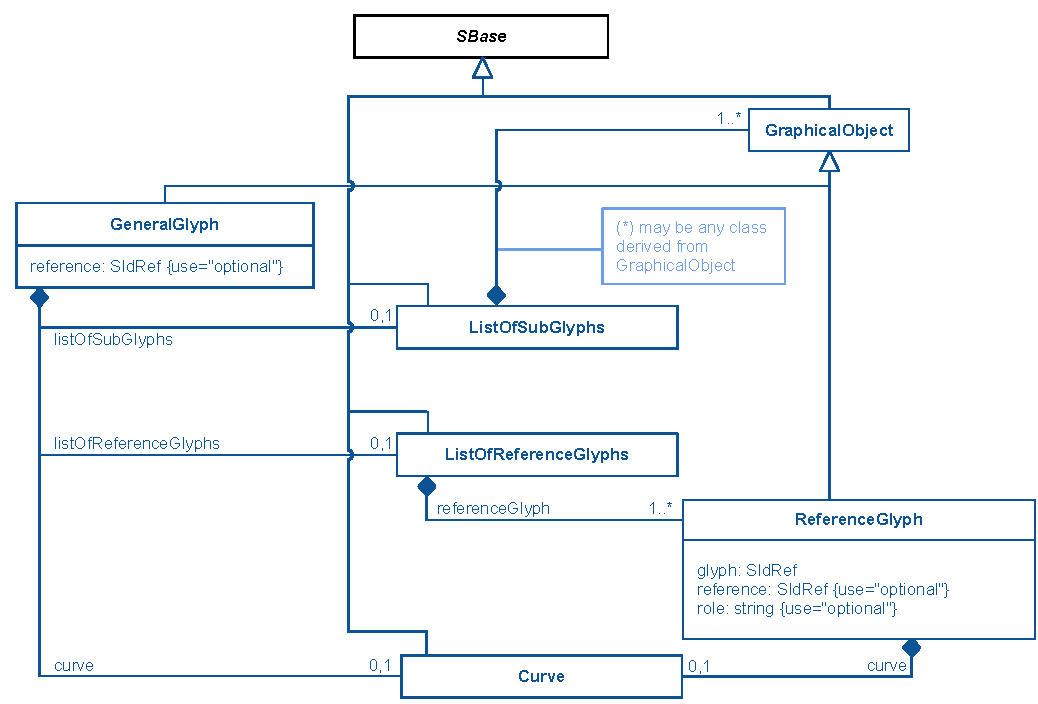
\includegraphics[scale=0.9]{uml/layout-generalglyph-model-uml}\\
\label{uml:generalglyph}
\caption{The definitions of the \GeneralGlyph class.}
\end{figure}

\paragraph{The \token{reference} attribute}
The optional \token{reference} attribute of type \primtype{SIdRef} that 
can be used to specify the \token{id} of the corresponding element in 
the model that is represented. 


\paragraph {The \token{listOfSubGlyphs} element}
\label{listofsubglyphs-class}
The \ListOfSubGlyphs is optional. It is a list of \GraphicalObject or 
derived classes. When present it must contain at least one such element. 

Unlike the \ListOfAdditionalGraphicalObjects in the \LayoutClass class, 
the \token{listOfSubGlyphs} may contain any derived class, such as for 
example \TextGlyph elements. 


\paragraph {The \token{listOfReferenceGlyphs} element}
\label{listofreferenceglyphs-class}
The \ListOfReferenceGlyphs is optional, since conceivably the \GeneralGlyph could just contain a number of sub glyphs. When present, it must include at least one \ReferenceGlyph. 


\paragraph {The \token{curve} element}
The optional \Curve element (\ref{curve-class}) can be used to describe 
a curve representation for the \GeneralGlyph. 

If a \GeneralGlyph specifies a curve, the bounding box is to be ignored. 

\subsubsection{The ReferenceGlyph class}
\label{referenceglyph-class}
The \token{referenceGlyph} element describes the graphical connection 
between an arbitrary \GraphicalObject (or derived element) and a 
\GeneralGlyph (which would be an arrow or some curve in most cases). 

As can be seen in the diagram \ref{uml:generalglyph}, a \ReferenceGlyph 
inherits from \GraphicalObject. Additionally it has a mandatory 
attribute \token{glyph} and two optional attributes \token{reference} 
and \token{role}. Optionally the \ReferenceGlyph also has an element 
\token{curve}. 

The ReferenceGlyph should either contain a bounding box or a curve 
specification, if both are given, the bounding box should be ignored. 

\paragraph{The \token{glyph} attribute}
The \token{glyph} is of type \primtype{SIdRef}. It contains a reference 
to the \token{id} of a \GraphicalObject (or derived) object that is to 
be connected to the \GeneralGlyph. 

This attribute is mandatory so as to ensure unambiguously which glyph has to be 
connected with this GeneralGlyph. 


\paragraph{The \token{reference} attribute}
The \token{reference} is an optional attribute of type \primtype{SIdRef} 
that is used to connect the \ReferenceGlyph with a element of the 
containing SBML model. 

\paragraph{The \token{role} attribute}
The \token{role} attribute is of type \primtype{string} and is used to 
specify how the reference should be displayed. 

While as \primtype{string}, the value of the \token{role} attribute is unconstraint, 
current implementations use the same values as specified in \ref{speciesreferencerole-type}.

\paragraph{The \token{curve} element}
The \token{curve} is an optional element of type \Curve. When present 
the glyph's bounding box (as inherited from the \GraphicalObject) is to 
be disregarded. 

So as to make the drawing of these curves as easy as possible the line 
segments should be ordered depending on the role of the \ReferenceGlyph:

\begin{itemize}
	\item If the glyph represents a modification it should start at the glyph and end at the center of the \GeneralGlyph.
	\item otherwise it should begin at the center section of the \GeneralGlyph and end at the reference glyph. 
\end{itemize}


\subsection{The TextGlyph class}
\label{textglyph-class}
The \TextGlyph class describes the position and dimension of text 
labels. It inherits from \GraphicalObject and adds the attributes 
\token{graphicalObject}, \token{text} and \token{originOfText}. 


For an example see \ref{example:textglyph}.

\begin{figure}[!h]
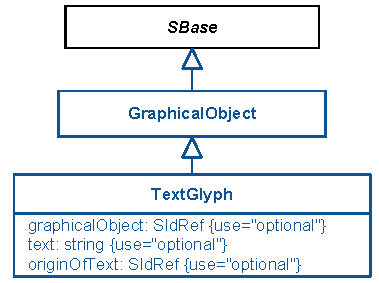
\includegraphics{uml/layout-textglyph-uml}\\
\caption{The definitions of the \TextGlyph class.}
\label{uml:textglyph}
\end{figure}

\paragraph{The \token{graphicalObject} attribute}
The attribute \token{graphicalObject} is of type \primtype{SIdRef}. It 
contains the \token{id} of any \GraphicalObject and specifies that the 
\TextGlyph should be considered to be a label to that object. This 
allows modelers to indicate that the label is to be moved together with the 
object. 

\paragraph{The \token{text} attribute}
The optional \token{text} attribute is of type \primtype{string}. It 
facilitates adding of independent text, like a title or a comment to the 
diagram. 

\paragraph{The \token{originOfText} attribute}
Additionally the optional attribute \token{originOfText} of type 
\primtype{SIdRef} can hold the \token{id} of an entity in the SBML 
model. If it is specified, the text to be displayed is taken from the 
\token{name} attribute of the referenced object. 

If both attributes \token{originOfText} and \token{text} are specified, 
the \token{text} attribute overrides the \\ \token{originOfText}. 


